\section{Transitioning to Three Dimensions}
The move to 3D was slow, the jump from \emph{pygame} to a full blown physics simulation was a big leap and it came with its problems.

\subsection{CoppeliaSim and RLBench}

CoppeliaSim is a mostly open source simulation program that provides full access to its features through an educational license and RLBench \cite{james2019rlbenchrobotlearningbenchmark} is an in-house (Imperial) tool adapted to plug into CoppeliaSim through its python API interface, PyRep \cite{pyrep2020}. There are many tutorials online to help learn how CoppeliaSim operates and designing some scenes. However, RLBench is a harder beast to tame. Although the system is very smart and it eliminates a lot of the required manual work before starting experimenting; it is quite old, plugs into version $4.1$ of CoppeliaSim from 2020. As well as its age, I had had some issues setting it up on my system. 

\subsection{Environment Issues}\todo[color=red]{this section might need shortening, 2 pages is a lot for this}
One of the first large-scale issues I'd face in this project came quite early in its lifespan. I would soon learn robotics development is mostly done on Linux based machines and the journey to getting everything working would be quite long.

\begin{itemize}
  \item\textbf{WSL Setup.}
  I thought this wouldn't be a problem, as WSL version 2 has been pretty good with GUI applications running on Linux and thought I could run Coppelia on there and still access any GUI (Graphical User Interface) I might need while developing tasks and observing my robot. The translation layer between the operating systems might cause some slowing but there shouldn't be any major issues. Upon configuring everything as the installation guide suggested in RLBench and PyRep repositories. I had few issues linking object files downloaded with CoppeliaSim into the PyRep layer. I had some issues with object files, and it was a WSL issue.

  \item\textbf{Linux Virtual Machine.}
  As RLBench suggested Debian based systems, and seeing the tutorials were done on Ubuntu, I created a Virtual Machine running it. Though, the rendering of Virtual Box was definitely going through some sort of translation through Windows and the GPU adapter was not linking properly. So, everything was extremely sluggish, and running the non-primitive examples even crashed my virtual machine instances a few times.

  \item\textbf{Dual Booting.}
  I had some issues partitioning the drive Windows was already installed, so decided to get myself another drive I could boot Ubuntu from. After running through the same setup steps and linking binaries, I was finally running RLBench. With one caveat, CoppeliaSim constantly complained that I was missing some video compression libraries; though seemed to work perfectly fine after installing them. It would always complain to me with a pop-up (see Figure \ref{fig:missing-libs}) but I found no issues with it during the project.

  \item\textbf{Side Note on Campus Machines.}
  I knew that a solution to all of my problems might have been using a machine at the labs. I thought an issue with that may have been that RLBench needs some binary linking and setting of system variables, and my personal machine is plenty powerful for a ML project, and observing agents seemed important to this project to I stuck to my personal machine
\end{itemize}

\subsubsection{RLBench Usability Issues}
As I started using RLBench other issues started popping up, PyRep was randomly failing calls to CoppeliaSim due to errors raised in RLBench due to unexpected types and hitting exceptions such as \emph{``Should not be here''}, the simulator would constantly and seemingly randomly crash, data from observations and other live elements within the simulator would give bogus data, like it being randomly \verb|None| or empty arrays.which was especially frustrating. 

\subsubsection{PyBullet}
The first option was PyBullet \cite{pybullet}, an open-source Python module for simulation, it wraps the Bullet SDK \cite{bullet3} and provides a completely customisable simulation experience. Though, the GUI experience is lacking and almost everything is controlled through the SDK's C-API.

Following some rough tutorials and combing through the manual for the module, I was able to put together fairly simple graphics and shapes to start creating some tasks. Although, I came to a halting realisation soon after. Which was that without a complete robot learning suite at my disposal I would need to figure out a lot of the systems from scratch. Such as camera placements and movement systems, seamless task creation and linking, environment management, demonstrations and so on.
\\\\
So the main dilemma was, should I be wasting time making a comprehensive suite to fit my needs early on in the project before  continuing with the premise of the task, or stick with RLBench and solve issues as they arise. As RLBench is open-source and some projects out there use it I thought I'd stick this this toolkit.

\section{First Steps in 3D: Reaching Task}\label{sec:3d-reaching-tasks}
Now deciding to stick with RLBench, the very first step was to translate the 2D task I played with earlier, \ref{subsec:ew-2d-problem}, into a 3D setting. So, the simple reaching task was made. 

\subsection{Designing the Task}
RLBench provides an intuitive method for quickly creating and validating tasks. Following the tutorials provided by the creator of RLBench and other resources online on CoppeliaSim \todo{link some copsim manuals or information here.} I could now create tasks for my use case.

Tasks are created using the \emph{`task builder'} CLI \ref{fig:task-builder}, which is a user facing interface that talks to the PyRep API which in turn controls CoppeliaSim. This allows the user to use GUI elements within the simulator to create objects, boundaries as well as edit their properties while observing what they look like in different camera view layers. Then the scene is wired using the automatically created \verb|Task| class. Where \emph{initialisation}, \emph{episode step} and other task related systems can be altered for a \verb|Scene| object to then use.

\begin{figure}[htbp]
  \centering
  \begin{subfigure}{0.40\linewidth}
    \centering
    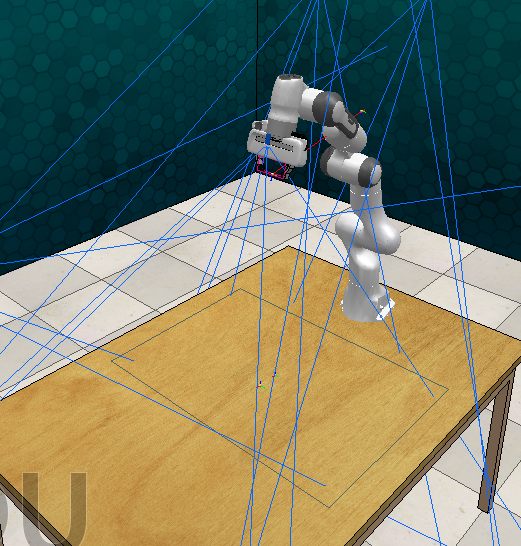
\includegraphics[width=0.4\linewidth]{assets/early-work/task-builder-scene.png}
    \caption{Simulator: Graphical view of the new task}
  \end{subfigure}%
  \begin{subfigure}{0.40\linewidth}
    \centering
    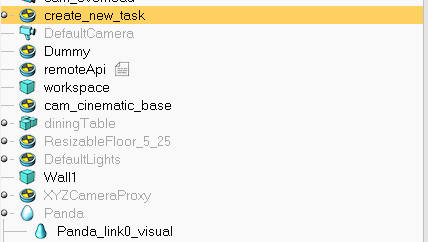
\includegraphics[width=0.6\linewidth]{assets/early-work/task-builder-scene-hierarchy.png}
    \caption{Simulator: Scene Hierarchy of the objects in the new task}
  \end{subfigure}
  \caption{Creating a new task with `task builder'}\label{fig:task-builder}
\end{figure}

The reaching task is simple, see Figure \ref{fig:reach-no-obs}. I decided to use the \emph{Panda arm}, as that seemed to be standard and more importantly immediately supported by RLBench. It has 7 Degrees of Freedom (DoF) and a gripper -so the action space is a 8 dimensional vector. Then a red spherical target, which is not tangible. It will be visually rendered, so the cameras can observe it, however, the arm cannot collide or interact with it physically. Finally, added a proximity sensor to the target (not rendered) so the task can be immediately classified as completed.

% //NOTE: relative paths for images, maybe add submodule once project is finished
\begin{figure}[htbp]
  \centering
  \begin{subfigure}{0.30\linewidth}
    \centering
    \includegraphics[width=0.5\linewidth]{../fyp/assets/task-pics/reach-no-obs/random-front.png}      
    \caption{Front View}
  \end{subfigure}%
  \hfill
  \begin{subfigure}{0.30\linewidth}
    \centering
    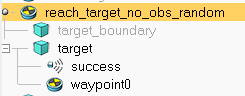
\includegraphics[width=0.8\linewidth]{assets/early-work/random-scene-hierarchy.png}
    \caption{Scene Hierarchy}\label{fig:reach-no-obs-hierarchy}
  \end{subfigure}%
  \hfill
  \begin{subfigure}{0.30\linewidth}
    \centering
    \includegraphics[width=0.5\linewidth]{../fyp/assets/task-pics/reach-no-obs/random-top.png}
    \caption{Top View}
  \end{subfigure}
  \caption{Reaching Task with no obstacles}\label{fig:reach-no-obs}
\end{figure}

\subsection{Setting up the Environment}
The \verb|Environment| is the all encompassing medium where the simulation happens. It contains the information about the scene, the robot: its movement system and control mechanism; and what can be observed. The environment is kept consistent throughout the project, see \ref{lst:env-setup}. We can control the stepping action requires for the robot to move. I opted for velocity control and arbitrarily decided to apply the gripper movement once the movement was completed.

This doesn't affect the design of policies in any way, as all the demonstrations were collected in the same environment, and the labelled data will be of the same kind. The \verb|dataset_root| points to where to load demonstrations from given a task \ref{subsec:saving-demos}. Different tasks can be loaded on the same active environment, though not at the same time. Finally, the observation config, which control what should be recorded and can be later accessible from the root as well as the size of the rgb cameras in terms of pixel resolution. Other cameras and sensors can be enabled and disabled using the \verb|CameraConfig| as shown in the code snippet \ref{lst:env-setup}; as well as the rest of the launching process.

\subsubsection{RLBench Demonstrations}
Demonstrations are provided encapsulated in a \verb|Demo| class and contain a series of observations (belonging to a class \verb|Observation|). These include state information of the robot and the environment, such as sensor and camera readings; which need to be configured when the environment is started. This modular approach means I can collect demonstrations, then selectively choose what to use, for example, ignore a camera or a sensor. \par 
Demonstrations are created following waypoints. PyRep expects  \verb|Dummy| objects within the scene called ``waypoint$x$'' where sequence number of the waypoint starting from $0$. Then the demonstration engine calculates trajectories to these waypoints in sequence. For example, in Figure \ref{fig:reach-no-obs-hierarchy}, we have `waypoint0' within the target, for which a trajectory will be calculated from the tip of the robot gripper.

By default the demonstrations -which I will refer to as ``demos'' from now on- and specifically the cameras pre-placed in the scene, produce images of resolution $128 \times 128$ pixels. I binned this down to $64 \times 64$. This comes in handy as I can keep the processing power low and can adapt the policy for higher resolution cameras by scaling it up later on. This resolution is an arbitrary choice and might need to increase the scale depending on feature extraction proficiency and whether I can identify this to be a limiting factor to learning a task.

\subsubsection{Saving Demonstrations}\label{subsec:saving-demos}
Final part of the environment is to save demonstrations. To evaluate different policies fairly, I will train them on the same data, as well as control any random seeds. RLBench provides an interface to save and load demos. However, they do it in an episodic and a slightly convoluted way; for tasks that have clearly defined episodes and variations. I have slightly altered the saving and loading code to easily integrate them into my work. I have also recorded all the sensor and all the cameras in these demos, just in case they might be required later in the project.

